\chapter{The Ball}

It was in the warmest days of July, when in due course of time the
Saturday arrived upon which the ball was to take place at M. de
Morcerf’s. It was ten o’clock at night; the branches of the great trees
in the garden of the count’s house stood out boldly against the azure
canopy of heaven, which was studded with golden stars, but where the
last fleeting clouds of a vanishing storm yet lingered.

From the apartments on the ground floor might be heard the sound of
music, with the whirl of the waltz and galop, while brilliant streams
of light shone through the openings of the Venetian blinds. At this
moment the garden was only occupied by about ten servants, who had just
received orders from their mistress to prepare the supper, the serenity
of the weather continuing to increase. Until now, it had been undecided
whether the supper should take place in the dining-room, or under a
long tent erected on the lawn, but the beautiful blue sky, studded with
stars, had settled the question in favor of the lawn.

The gardens were illuminated with colored lanterns, according to the
Italian custom, and, as is usual in countries where the luxuries of the
table—the rarest of all luxuries in their complete form—are well
understood, the supper-table was loaded with wax-lights and flowers.

\begin{figure}[ht]
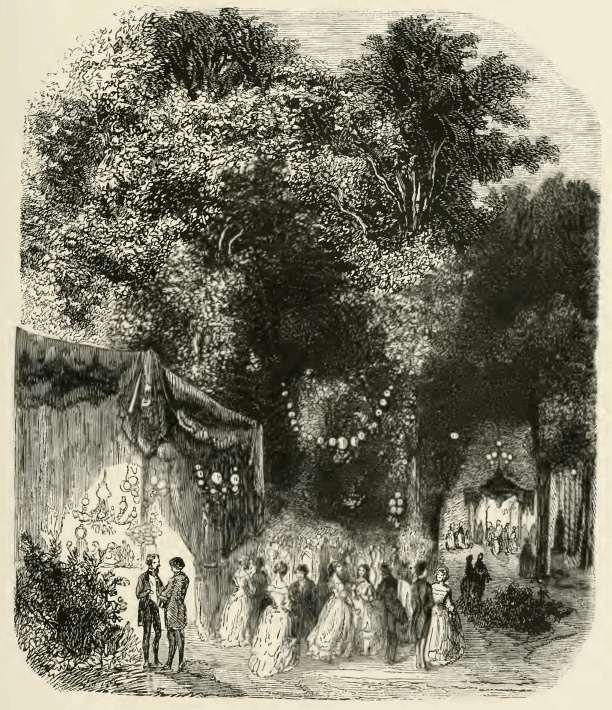
\includegraphics[width=\textwidth]{30297m.jpg}
\end{figure}

At the time the Countess of Morcerf returned to the rooms, after giving
her orders, many guests were arriving, more attracted by the charming
hospitality of the countess than by the distinguished position of the
count; for, owing to the good taste of Mercédès, one was sure of
finding some devices at her entertainment worthy of describing, or even
copying in case of need.

Madame Danglars, in whom the events we have related had caused deep
anxiety, had hesitated about going to Madame de Morcerf’s, when during
the morning her carriage happened to meet that of Villefort. The latter
made a sign, and when the carriages had drawn close together, said:

“You are going to Madame de Morcerf’s, are you not?”

“No,” replied Madame Danglars, “I am too ill.”

“You are wrong,” replied Villefort, significantly; “it is important
that you should be seen there.”

“Do you think so?” asked the baroness.

“I do.”

“In that case I will go.”

And the two carriages passed on towards their different destinations.
Madame Danglars therefore came, not only beautiful in person, but
radiant with splendor; she entered by one door at the time when
Mercédès appeared at the door. The countess took Albert to meet Madame
Danglars. He approached, paid her some well merited compliments on her
toilet, and offered his arm to conduct her to a seat. Albert looked
around him.

“You are looking for my daughter?” said the baroness, smiling.

“I confess it,” replied Albert. “Could you have been so cruel as not to
bring her?”

“Calm yourself. She has met Mademoiselle de Villefort, and has taken
her arm; see, they are following us, both in white dresses, one with a
bouquet of camellias, the other with one of myosotis. But tell me——”

“Well, what do you wish to know?”

“Will not the Count of Monte Cristo be here tonight?”

“Seventeen!” replied Albert.

“What do you mean?”

“I only mean that the count seems the rage,” replied the viscount,
smiling, “and that you are the seventeenth person that has asked me the
same question. The count is in fashion; I congratulate him upon it.”

“And have you replied to everyone as you have to me?”

“Ah, to be sure, I have not answered you; be satisfied, we shall have
this ‘lion’; we are among the privileged ones.”

“Were you at the Opera yesterday?”

“No.”

“He was there.”

“Ah, indeed? And did the eccentric person commit any new originality?”

“Can he be seen without doing so? Elssler was dancing in \textit{Le Diable
boiteux}; the Greek princess was in ecstasies. After the cachucha he
placed a magnificent ring on the stem of a bouquet, and threw it to the
charming danseuse, who, in the third act, to do honor to the gift,
reappeared with it on her finger. And the Greek princess,—will she be
here?”

“No, you will be deprived of that pleasure; her position in the count’s
establishment is not sufficiently understood.”

“Wait; leave me here, and go and speak to Madame de Villefort, who is
trying to attract your attention.”

Albert bowed to Madame Danglars, and advanced towards Madame de
Villefort, whose lips opened as he approached.

“I wager anything,” said Albert, interrupting her, “that I know what
you were about to say.”

“Well, what is it?”

“If I guess rightly, will you confess it?”

“Yes.”

“On your honor?”

“On my honor.”

“You were going to ask me if the Count of Monte Cristo had arrived, or
was expected.”

“Not at all. It is not of him that I am now thinking. I was going to
ask you if you had received any news of Monsieur Franz.”

“Yes,—yesterday.”

“What did he tell you?”

“That he was leaving at the same time as his letter.”

“Well, now then, the count?”

“The count will come, of that you may be satisfied.”

“You know that he has another name besides Monte Cristo?”

“No, I did not know it.”

“Monte Cristo is the name of an island, and he has a family name.”

“I never heard it.”

“Well, then, I am better informed than you; his name is Zaccone.”

“It is possible.”

“He is a Maltese.”

“That is also possible.

“The son of a shipowner.”

“Really, you should relate all this aloud, you would have the greatest
success.”

“He served in India, discovered a mine in Thessaly, and comes to Paris
to establish a mineral water-cure at Auteuil.”

“Well, I’m sure,” said Morcerf, “this is indeed news! Am I allowed to
repeat it?”

“Yes, but cautiously, tell one thing at a time, and do not say I told
you.”

“Why so?”

“Because it is a secret just discovered.”

“By whom?”

“The police.”

“Then the news originated——”

“At the prefect’s last night. Paris, you can understand, is astonished
at the sight of such unusual splendor, and the police have made
inquiries.”

“Well, well! Nothing more is wanting than to arrest the count as a
vagabond, on the pretext of his being too rich.”

“Indeed, that doubtless would have happened if his credentials had not
been so favorable.”

“Poor count! And is he aware of the danger he has been in?”

“I think not.”

“Then it will be but charitable to inform him. When he arrives, I will
not fail to do so.”

Just then, a handsome young man, with bright eyes, black hair, and
glossy moustache, respectfully bowed to Madame de Villefort. Albert
extended his hand.

“Madame,” said Albert, “allow me to present to you M. Maximilian
Morrel, captain of Spahis, one of our best, and, above all, of our
bravest officers.”

“I have already had the pleasure of meeting this gentleman at Auteuil,
at the house of the Count of Monte Cristo,” replied Madame de
Villefort, turning away with marked coldness of manner.

This answer, and especially the tone in which it was uttered, chilled
the heart of poor Morrel. But a recompense was in store for him;
turning around, he saw near the door a beautiful fair face, whose large
blue eyes were, without any marked expression, fixed upon him, while
the bouquet of myosotis was gently raised to her lips.

The salutation was so well understood that Morrel, with the same
expression in his eyes, placed his handkerchief to his mouth; and these
two living statues, whose hearts beat so violently under their marble
aspect, separated from each other by the whole length of the room,
forgot themselves for a moment, or rather forgot the world in their
mutual contemplation. They might have remained much longer lost in one
another, without anyone noticing their abstraction. The Count of Monte
Cristo had just entered.

We have already said that there was something in the count which
attracted universal attention wherever he appeared. It was not the
coat, unexceptional in its cut, though simple and unornamented; it was
not the plain white waistcoat; it was not the trousers, that displayed
the foot so perfectly formed—it was none of these things that attracted
the attention,—it was his pale complexion, his waving black hair, his
calm and serene expression, his dark and melancholy eye, his mouth,
chiselled with such marvellous delicacy, which so easily expressed such
high disdain,—these were what fixed the attention of all upon him.

Many men might have been handsomer, but certainly there could be none
whose appearance was more \textit{significant}, if the expression may be used.
Everything about the count seemed to have its meaning, for the constant
habit of thought which he had acquired had given an ease and vigor to
the expression of his face, and even to the most trifling gesture,
scarcely to be understood. Yet the Parisian world is so strange, that
even all this might not have won attention had there not been connected
with it a mysterious story gilded by an immense fortune.

\begin{figure}[ht]
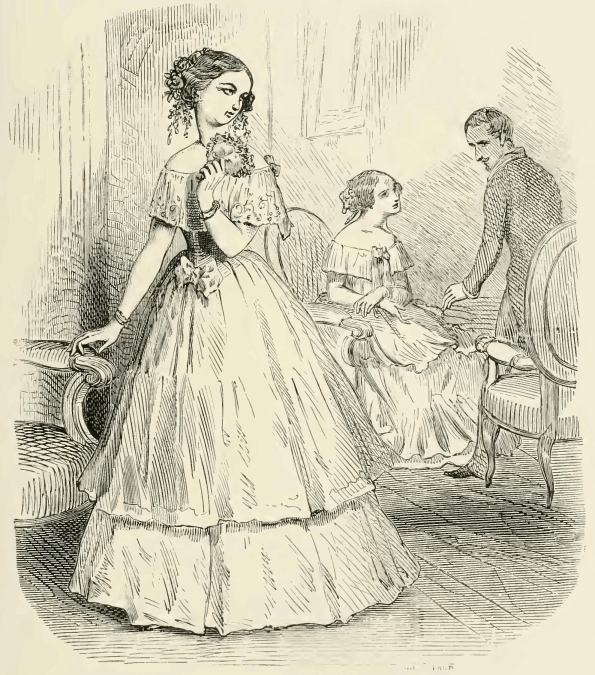
\includegraphics[width=\textwidth]{30301m.jpg}
\end{figure}

Meanwhile he advanced through the assemblage of guests under a battery
of curious glances towards Madame de Morcerf, who, standing before a
mantle-piece ornamented with flowers, had seen his entrance in a
looking-glass placed opposite the door, and was prepared to receive
him. She turned towards him with a serene smile just at the moment he
was bowing to her. No doubt she fancied the count would speak to her,
while on his side the count thought she was about to address him; but
both remained silent, and after a mere bow, Monte Cristo directed his
steps to Albert, who received him cordially.

“Have you seen my mother?” asked Albert.

“I have just had the pleasure,” replied the count; “but I have not seen
your father.”

“See, he is down there, talking politics with that little group of
great geniuses.”

“Indeed?” said Monte Cristo; “and so those gentlemen down there are men
of great talent. I should not have guessed it. And for what kind of
talent are they celebrated? You know there are different sorts.”

“That tall, harsh-looking man is very learned, he discovered, in the
neighborhood of Rome, a kind of lizard with a vertebra more than
lizards usually have, and he immediately laid his discovery before the
Institute. The thing was discussed for a long time, but finally decided
in his favor. I can assure you the vertebra made a great noise in the
learned world, and the gentleman, who was only a knight of the Legion
of Honor, was made an officer.”

“Come,” said Monte Cristo, “this cross seems to me to be wisely
awarded. I suppose, had he found another additional vertebra, they
would have made him a commander.”

“Very likely,” said Albert.

“And who can that person be who has taken it into his head to wrap
himself up in a blue coat embroidered with green?”

“Oh, that coat is not his own idea; it is the Republic’s, which deputed
David\footnote[12]{Jacques-Louis David, a famous French painter (1748-1825).}
to devise a uniform for the Academicians.”

“Indeed?” said Monte Cristo; “so this gentleman is an Academician?”

“Within the last week he has been made one of the learned assembly.”

“And what is his especial talent?”

“His talent? I believe he thrusts pins through the heads of rabbits, he
makes fowls eat madder, and punches the spinal marrow out of dogs with
whalebone.”

“And he is made a member of the Academy of Sciences for this?”

“No; of the French Academy.”

“But what has the French Academy to do with all this?”

“I was going to tell you. It seems——”

“That his experiments have very considerably advanced the cause of
science, doubtless?”

“No; that his style of writing is very good.”

“This must be very flattering to the feelings of the rabbits into whose
heads he has thrust pins, to the fowls whose bones he has dyed red, and
to the dogs whose spinal marrow he has punched out?”

Albert laughed.

“And the other one?” demanded the count.

“That one?”

“Yes, the third.”

“The one in the dark blue coat?”

“Yes.”

“He is a colleague of the count, and one of the most active opponents
to the idea of providing the Chamber of Peers with a uniform. He was
very successful upon that question. He stood badly with the Liberal
papers, but his noble opposition to the wishes of the court is now
getting him into favor with the journalists. They talk of making him an
ambassador.”

\begin{figure}[ht]
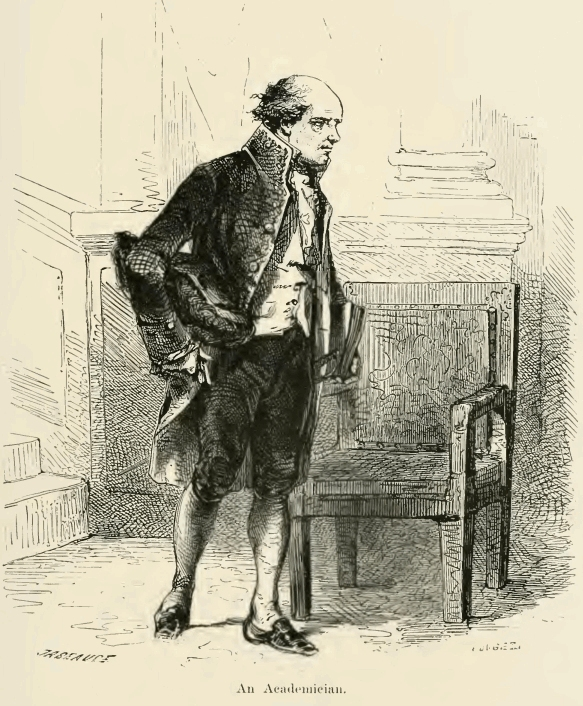
\includegraphics[width=\textwidth]{30303m.jpg}
\end{figure}

“And what are his claims to the peerage?”

“He has composed two or three comic operas, written four or five
articles in the \textit{Siècle}, and voted five or six years on the
ministerial side.”

“Bravo, viscount,” said Monte Cristo, smiling; “you are a delightful
\textit{cicerone}. And now you will do me a favor, will you not?”

“What is it?”

“Do not introduce me to any of these gentlemen; and should they wish
it, you will warn me.” Just then the count felt his arm pressed. He
turned round; it was Danglars.

“Ah! is it you, baron?” said he.

“Why do you call me baron?” said Danglars; “you know that I care
nothing for my title. I am not like you, viscount; you like your title,
do you not?”

“Certainly,” replied Albert, “seeing that without my title I should be
nothing; while you, sacrificing the baron, would still remain the
millionaire.”

“Which seems to me the finest title under the royalty of July,” replied
Danglars.

“Unfortunately,” said Monte Cristo, “one’s title to a millionaire does
not last for life, like that of baron, peer of France, or academician;
for example, the millionaires Franck \& Poulmann, of Frankfurt, who have
just become bankrupts.”

“Indeed?” said Danglars, becoming pale.

“Yes; I received the news this evening by a courier. I had about a
million in their hands, but, warned in time, I withdrew it a month
ago.”

“Ah, \textit{mon Dieu!}” exclaimed Danglars, “they have drawn on me for
200,000 francs!”

“Well, you can throw out the draft; their signature is worth five per
cent.”

“Yes, but it is too late,” said Danglars, “I have honored their bills.”

“Then,” said Monte Cristo, “here are 200,000 francs gone after——”

“Hush, do not mention these things,” said Danglars; then, approaching
Monte Cristo, he added, “especially before young M. Cavalcanti;” after
which he smiled, and turned towards the young man in question.

Albert had left the count to speak to his mother, Danglars to converse
with young Cavalcanti; Monte Cristo was for an instant alone. Meanwhile
the heat became excessive. The footmen were hastening through the rooms
with waiters loaded with ices. Monte Cristo wiped the perspiration from
his forehead, but drew back when the waiter was presented to him; he
took no refreshment. Madame de Morcerf did not lose sight of Monte
Cristo; she saw that he took nothing, and even noticed his gesture of
refusal.

“Albert,” she asked, “did you notice that?”

“What, mother?”

“That the count has never been willing to partake of food under the
roof of M. de Morcerf.”

“Yes; but then he breakfasted with me—indeed, he made his first
appearance in the world on that occasion.”

“But your house is not M. de Morcerf’s,” murmured Mercédès; “and since
he has been here I have watched him.”

“Well?”

“Well, he has taken nothing yet.”

“The count is very temperate.”

Mercédès smiled sadly.

“Approach him,” said she, “and when the next waiter passes, insist upon
his taking something.”

“But why, mother?”

“Just to please me, Albert,” said Mercédès. Albert kissed his mother’s
hand, and drew near the count. Another salver passed, loaded like the
preceding ones; she saw Albert attempt to persuade the count, but he
obstinately refused. Albert rejoined his mother; she was very pale.

“Well,” said she, “you see he refuses?”

“Yes; but why need this annoy you?”

“You know, Albert, women are singular creatures. I should like to have
seen the count take something in my house, if only an ice. Perhaps he
cannot reconcile himself to the French style of living, and might
prefer something else.”

“Oh, no; I have seen him eat of everything in Italy; no doubt he does
not feel inclined this evening.”

“And besides,” said the countess, “accustomed as he is to burning
climates, possibly he does not feel the heat as we do.”

“I do not think that, for he has complained of feeling almost
suffocated, and asked why the Venetian blinds were not opened as well
as the windows.”

“In a word,” said Mercédès, “it was a way of assuring me that his
abstinence was intended.”

And she left the room.

A minute afterwards the blinds were thrown open, and through the
jessamine and clematis that overhung the window one could see the
garden ornamented with lanterns, and the supper laid under the tent.
Dancers, players, talkers, all uttered an exclamation of joy—everyone
inhaled with delight the breeze that floated in. At the same time
Mercédès reappeared, paler than before, but with that imperturbable
expression of countenance which she sometimes wore. She went straight
to the group of which her husband formed the centre.

“Do not detain those gentlemen here, count,” she said; “they would
prefer, I should think, to breathe in the garden rather than suffocate
here, since they are not playing.”

“Ah,” said a gallant old general, who, in 1809, had sung \textit{Partant pour
la Syrie},—“we will not go alone to the garden.”

“Then,” said Mercédès, “I will lead the way.”

Turning towards Monte Cristo, she added, “count, will you oblige me
with your arm?”

The count almost staggered at these simple words; then he fixed his
eyes on Mercédès. It was only a momentary glance, but it seemed to the
countess to have lasted for a century, so much was expressed in that
one look. He offered his arm to the countess; she took it, or rather
just touched it with her little hand, and they together descended the
steps, lined with rhododendrons and camellias. Behind them, by another
outlet, a group of about twenty persons rushed into the garden with
loud exclamations of delight.
